\documentclass[12pt,a4paper]{report}
\usepackage[top=3cm, bottom=3.2cm, left=4cm, right=3cm]{geometry}
\usepackage{hyperref}
\usepackage{algorithmic}
\usepackage{graphicx}
\usepackage{cite}
\usepackage{setspace}
\usepackage{times}
\usepackage{tabulary}
\usepackage{xcolor}
\usepackage{multirow}
\usepackage[all]{hypcap}
\usepackage{tikz}
\usetikzlibrary{positioning}
% \usepackage{layout}
% \usepackage{showframe}
\hypersetup{
    pdftoolbar=true,        % show Acrobat’s toolbar?
    pdfmenubar=true,        % show Acrobat’s menu?
    pdffitwindow=false,     % window fit to page when opened
    pdfstartview={FitH},    % fits the width of the page to the window
    pdftitle={Modelling the Impact of Wind and EVs to the Power Grid in Orkney},    % title
    pdfauthor={Yifei Jing},     % author
    pdfsubject={Dissertation},   % subject of the document
    pdfcreator={Yifei Jing},   % creator of the document
    pdfproducer={Yifei Jing},
    pdfkeywords={Data Science} {Power grid} {Electrical vehicles} {Simulation},
    colorlinks,
    linkcolor=violet,
    citecolor=blue,
    urlcolor=brown
}
\def\BibTeX{{\rm B\kern-.05em{\sc i\kern-.025em b}\kern-.08em
    T\kern-.1667em\lower.7ex\hbox{E}\kern-.125emX}}
\pagenumbering{roman}
\begin{document}
    \onehalfspacing
    \title{\textbf{``Modelling the Impact of Wind and EVs to the Power Grid in Orkney''}}
    \author{by \\ \\ Yifei Jing \\ \\ An Honours report submitted for the Degree of: \\ \\
    BEng in Electrical and Electronic Engineering}
    \date{Feburary 2020}
    \maketitle
    % \layout{}

    \cleardoublepage  
    \phantomsection  
    \addcontentsline{toc}{chapter}{Table of Contents}
    \tableofcontents

    \cleardoublepage  
    \phantomsection  
    \addcontentsline{toc}{chapter}{List of Figures}
    \listoffigures

    \cleardoublepage  
    \phantomsection  
    \addcontentsline{toc}{chapter}{List of Tables}
    \listoftables
    \hyphenpenalty=100000
    \chapter*{Synopsis}
    \addcontentsline{toc}{chapter}{Synopsis}
        % A one page (two page max.) summary which briefly describes the report in a manner able to
        % be understood by an educated non-engineer.
        In this project, the impacts of EVs to the power grid in Orkeny, which has a large dependence on wind power, is analyzed from two perspectivs: grid storage and energy consumption.
        The storage works as a compensation for wind power generation, as it is an intermittent power resource. For different EVs penetrations, a viable range of the storage is analyzed. The consumption has an increasing tendency resulted from electrification on the island, which affects the relationship of electricity generation and demand. Additionally,
        some developed charging strategies which aims to increase robustness of grid are implemented to estimate their effects on storage and consumption. 

        The work is associated as: (1) Analysis collected data on total renewable power generation and demand to get relationships of loading profile, renewable generation and curtailments.
        (2) Design a small model of grid to simulate various EV penetrations, charging strategies, and curtailments.

        In work part (1), a data set is established to collect power and weather data from available data sources. Then, evaluations and analysis are performed on this data set.
        In work part (2), a model of grid is designed with \emph{C++} programming language base on a general simulation environment. To find optimized solution to the problems, \emph{Monte Carlo} simulation is used.

        
    \chapter*{Acknowledgements}
    \addcontentsline{toc}{chapter}{Acknowledgements}
        % The assistance that given to you.
    
    \chapter*{Statement of Authorship}
    \addcontentsline{toc}{chapter}{Statement of Authorship}

        I, Yifei Jing \\ \\ 
        State that this work submitted for assessment is my own and expressed in my own words.
        Any uses made within it of works of other authors in any form (eg. Ideas, figures, text, tables)
        are properly acknowledged at their point of use. A list of the references employed is included.
        \\ \\Date 
    \chapter*{Nomenclature}
    \addcontentsline{toc}{chapter}{Nomenclature}
    \chapter{Introduction}
    \pagenumbering{arabic}
    % This is chapter one, and in general it has three parts. Firstly, the objective of the project should be described. Secondly, a brief description, i.e. a few pages, should be given outlining how the project was tackled and what results were obtained. This can be viewed in two ways. The synopsis should have gained the reader’s attention, so this part can be regarded as expanding on the synopsis to further whet the reader’s appetite for the good things to come. Alternatively, this section can be considered to be a coherent presentation of summaries of each chapter. Finally, the introduction is a convenient place to discuss the uses or applications of the work done in the project.
        The increasing energy consumption against the ever-decreasing amount of
        energy resources like the oil and gas have led to
        growing concerns from the customers, governments, and researchers.
        Seeking for available solutions, renewable energy resources including
        photovoltaics (PV), wind, tidal, biomass and hydrogens have attracted
        more and more attention. Such renewable energy resources not only act as the substitution of the traditional power resources,
        but also have better performance on efficiency \footnote{The traditional power like the fossil fuel has only about 30\% overall efficiency from sources to end users, while the renewable energy resources have an about 70\% overall generation to grid connection efficiency. \cite{paper:renewableefficiency}}. 
        Having been providing 24\% power demand in 2017, the renewable power is assumed to increase to almost 30\% of power demand in 2023 \cite{website:iea}.
        Among these renewable power resources, wind power is a fast-growing
        renewable energy resource with a large number of wind turbines already
        installed in wind farms. 
        
        For those places with a typical strong windy climate but lack of fossil and gas production
        like Orkney, it is viable to connect wind generation to the grid for the sake of diminishing the budget on importing those non-renewable 
        energy resources and on the other hand achieving a further target of decarbonization. From this
        perspective, the community in Orkney is planning to eliminate the dependence on
        oil fuel and gas using completely clean electricity power resources like wind, hydrogen, and sunlight. 
        
        To increase wind generation capacity, an innovative Active Network Management (ANM) system was set up in 2009 to allow operators to connect wind farm generation to the grid \cite{website:ANM}. 
        Behold to ANM, the capacity of wind generation has been growing dramatically from 15.5 MW in 2009 to 47.7 MW in 2019 \cite{report:OrkneyAudit}, which is depicted in Fig \ref{fig_cummulative_wind_capacity}. 
        
        \begin{figure}[ht]
            \centerline{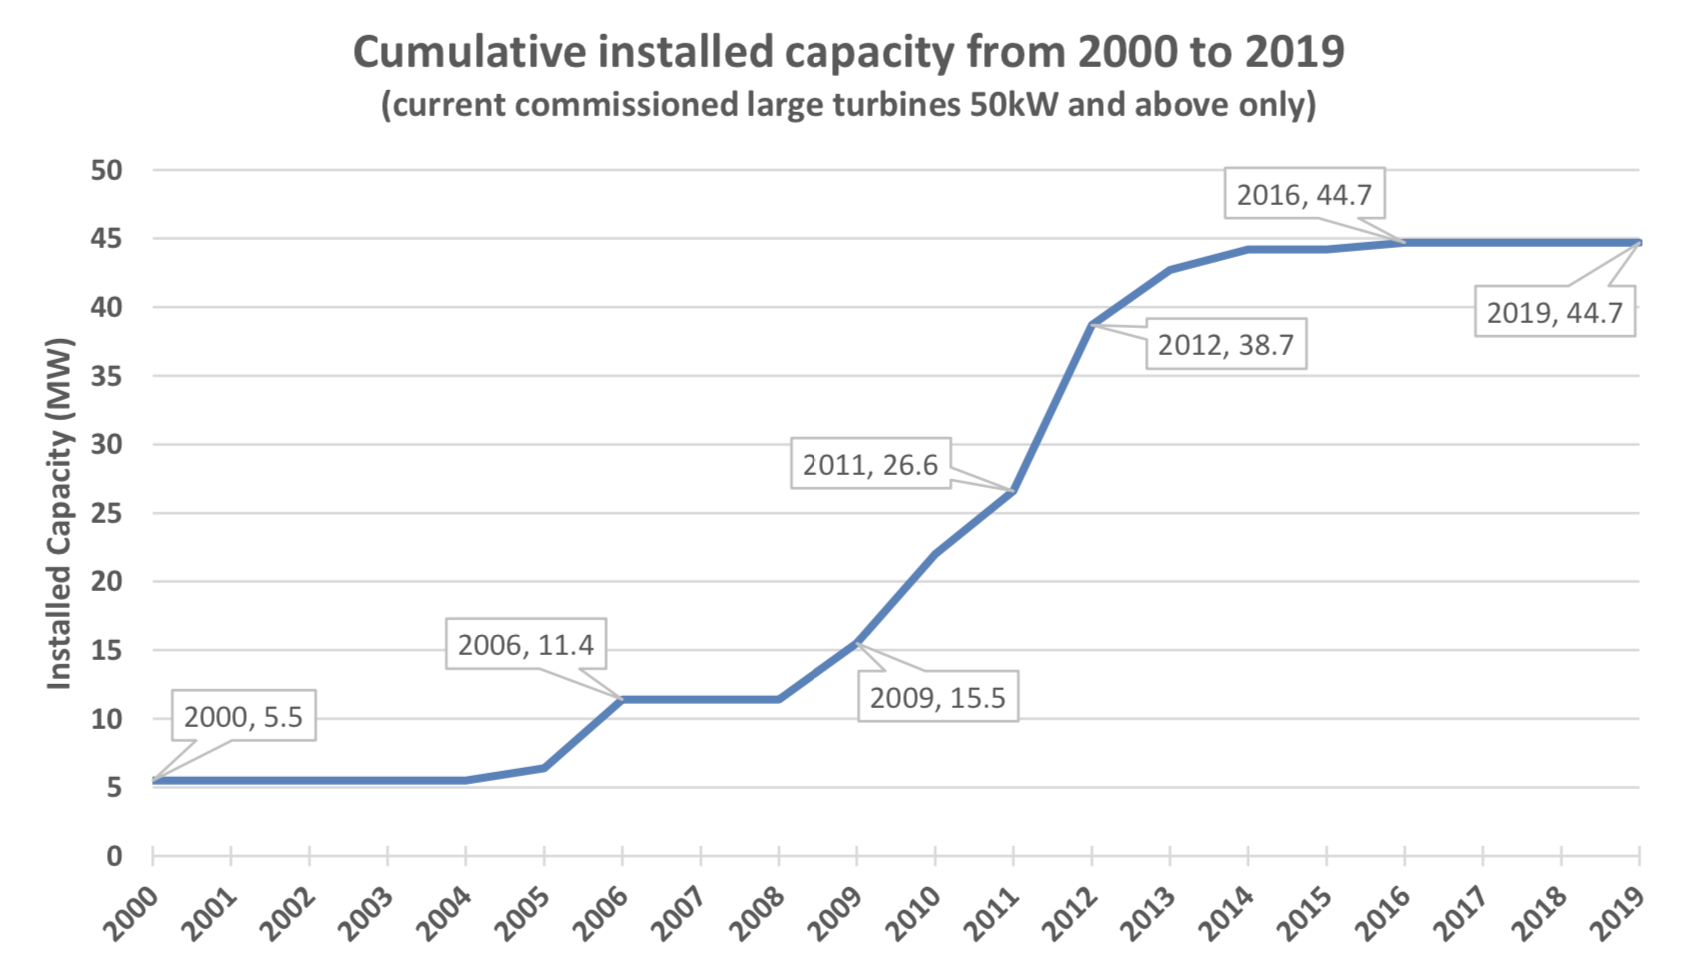
\includegraphics[scale=1]{cummulativewindcapacity}}
            \caption{The cummulative wind power generation capacity between 2000 and 2019}
            \label{fig_cummulative_wind_capacity}
        \end{figure}

        To increase hydropower capacity, a project called Surf`N'Turf was launched to build hydrogen storage in Eday, 
        which includes three tube trailers each capable of storing 250kg of hydrogen and one 500kg static hydrogen storage \cite{website:surfturf}. 

        In the past few years, some transitions of electrification have been posed; 
        like increasing the number of electrical vehicles (EVs) and ferries (EFs) to switch 
        from fossil demand to electricity demand, improving the gas heating types of 
        equipment to the electrical heating ones, and installing wind turbines with local 
        storage for households to achieve energy trades among customers. 
        Additionally, the number of EVs has been increasing drastically from a relatively small group to 234 in the first quarter of 2019 \cite{report:OrkneyAudit}, as is indicated in \hyperref[fig_EV_number]{Fig \ref*{fig_EV_number}}.
        The rate of growth is 975\% in 5 years. The reason of this high grow speed is that on the one hand distributed wind turbines and local energy reserve storage can be installed in Orkney, which increase the accessibility of electric power with cheaper price, on the other hand, the community of Orkney provides charging stations which can charge EVs without fee (This service was turned to be paid charging scheme in 2019 April \cite{report:OrkneyAudit}).

        \begin{figure}[ht]
            \centerline{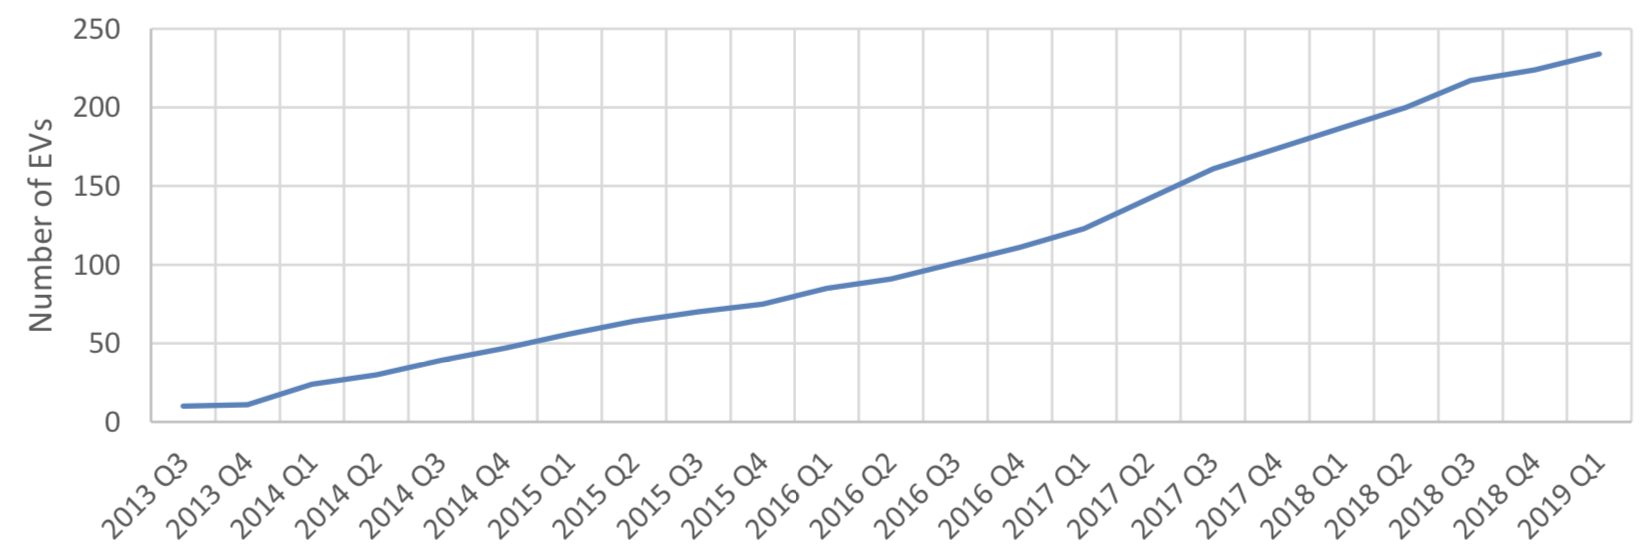
\includegraphics[scale=1]{evnumber}}
            \caption{The EV number evolution from 2013 to 2019}
            \label{fig_EV_number}
        \end{figure}

        However, some dilemmas have been introduced to the process of electrification. 
        These problems can be divided into two parts: storage and consumption.

        The energy storage system (ESS) installed in an electrical grid can provide various ancillary services as it is summarized in \cite{paper:Lawder2014}. 
        For wind power generation, because of its intermittent nature, the storage should be capable of providing regulation and compenstation for the gird \cite{paper:gridrisk} \cite{paper:gridscenarios}.
        Generally, the storage stores energy by recharging when the embedded renewable generation (ERG) is high and the demand is relatively low, 
        and it discharges when the demand is at peak value to avoid the cost of using expensive generators or imported energy. 
        If sometimes, the ERG reaches a point that the grid cannot keep the voltage below the maximum to sustain its stability, 
        the curtailment will happen, which causes the excess of output to be cut out by turning off some wind turbines. It is not possible to make profits 
        at this moment. 
        
        To solve this problem, the over generated energy can be exported to the mainland of UK via a 20MW transmission line \cite{book:Orkneypowerexport}. 
        However, there is still 16\% wind power generation having been curtailed in the last year \cite{report:OrkneyAudit}, which implies that the current wind power capacity has been excessive.
        
        On the other hand, when demand reaches the peak value of the day, but the ERG is at a low level, 
        it is expected the ESS will be capable of providing enough energy, whose capacity and technologies attach an important role on the period and frequency
        of provision. For example, the supercapacitor is capable of charging and discharging frequently, but it does not
        generally have large capacitance, thus it can only support services on short duration, the batteries like Li-ion, Ni-MH
        have larger capacitance, but limited life cycles which prevent them from switching between charging and discharging states
        frequntly. Because of the price issue, they are used for mid term duration and mostly on portable devices like mobile phones and
        EVs. For the gird, the storage used for frequency regulation and spinning reserve should be storage with small capacitance and longer cycle life, and for storage reservation, storage with large capacitance should be used.
        The characteristics of typical storage technologies are summarizes in \hyperref[table_storage_characteristics]{Table \ref*{table_storage_characteristics}} \cite{paper:Barton2004} \cite{paper:Vazquez2010}.
        
        Under the analysis of local power demand and generation, it is possible to estimate the amount of local storage in an appropriate range and determine its technique. 
        However, it is estimated that 99\% of the total power generation in Orkney is from the wind \cite{report:OrkneyAudit}, 
        which is intermittent in nature. Its large variance leads to an unstable connection to the grid, 
        which imposes large challenges to the design of the storage.

        In this project, the models of power demand and generation in Orkney from an over-all landscape will be first established based on available data collected from ANM \cite{website:ANM}. 
        Statistical features are extracted from these models and will be further discussed and compared with characteristics gathered from paper. 
        Later, a small grid model is designed to simulate with different storage capacities. 
        Problems on determining wind power generation and household demand models in this simulation model will also be mentioned. 
        To evaluate the performance of the storage in the grid, a metric will be defined and improved.

        \begin{table}[ht]
            \begin{tabulary}{\linewidth}{c L L L L}
                \hline
                Type & Energy efficiency (\%) & Energy density (Wh/kg) & Life cycle (cycles) & Services \\ \hline
                \hline
                Ni-Cd & 60 - 90 & 40 - 60 & 500 - 2000 & Wind power smoothing, spinning reserve \\ \hline
                Li-Ion & 70 - 85 & 100 - 200 & 500 - 2000 &  Wind power smoothing, spinning reserve, PV, portable devices\\ \hline
                Ni-MH & 50 - 80 & 60 - 80 & $<$ 3000 & Wind power smoothing, spinning reserve, PV, portable devices \\ \hline
                Pumped hydro & 65 - 80 & 0.3 & $>$ 20 years & Daily load cycle, weather variations \\ \hline
                Flywheel & 95 & 5 - 30 & $>$ 20000 &  Wind power smoothing, spinning reserve \\ \hline
                Supercapacitor & 100 & - & - & Voltage and frequency control, governor controlled generation \\ \hline
            \end{tabulary}
            \caption{Storage technologies and characteristics}
            \label{table_storage_characteristics}
        \end{table}
        
        The challenges on consumption derive mainly from its tendency of electrification as the EVs contribute a large amount of demand to the grid when being charged \cite{paper:PieltainFernandez2011}. 
        Generally, two charging modes are provided: 110V/15A as the normal mode and 240V/30A as the quick mode \cite{paper:Shao2010}. 
        From the ``Household Electricity Survey of UK'' \cite{report:household}, the peak load value of one household is generally happens at night, at about 700W which is lower than half of the charging power.
        Thus the challenges for the grid is to satisfy new peak demand resulting from increasing penetration of EVs.
        In this project, the effects of EV charging will be analyzed first from an over-all perspective based on three levels of penetration.
        Then different penetrations of EVs will be analyzed in the simulation framework established as a smaller replica of Orkney to determine optimal storage for the grid with high dependence on wind power. 
        After that, three charging strategies, which are summarized from \cite{paper:Qian2011}, will be implemented in this simulation model. Their effects on the grid demand profile and storage will be discussed.

        The results of this project should provide a good enough estimation of storage and demand in a power grid with a increasing penetration of EVs.
    \chapter{Background}
        In this section, the concepts and techniques in data analysis using in this project are provided. Then, a brief description of the simulation framework used to build the model is provided.

        \section{Statistical analysis}
        This section summaries concepts and tools used in statistical analysis. It starts from basic concepts, such as \emph{mean}, \emph{variance}, \emph{etc}, to multi-variate developments like \emph{covariance} and \emph{correlation}.
        \subsection{\emph{Mean, Variance, Min and Max}}
        The fundamental concepts of data analysis are: \emph{mean}, \emph{variance}, \emph{minimum} and \emph{maximum}. Assume the data in one dataset is described by a random variable $X$ and a distribution function $f(X)$ (It is better to form a discrete random varible than a continuous one, as it's probability function p.d. can directly represent the position of one sample $x$). 
        
        Then the \emph{mean} of it is defined as 
        \begin{equation}
            E(X) = \sum_{All\,\, x} x f(x)
            \label{formula_mean}
        \end{equation}

        It is a measure of the ``Central of gravity'' to one distribution derived from the fact that it is a sum of weighted samples in the distribution. Because of this, the \emph{Mean} can be affected by a very large value with small probability. Such is the case for the wind speed distribution analyzed in \hyperref[text_wind_speed_analysis]{Section \ref*{text_wind_speed_analysis}} that most of the wind speed is not large, but the mean is larger because of sevral extreme wind speed samples.

        Despite the influences by outliers in the \emph{Mean}, the \emph{Median} is introduced as the ``Central of location'' to one distribution, which is defined as the number m which satisfies:
        \begin{equation}
            Pr(X\leq m) \geq \frac{1}{2} \,\,\, and \,\,\, Pr(X\geq m) \geq \frac{1}{2}
        \end{equation}
        
        In practice, the two central properties both provide important information to the distribution.

        The \emph{Variance} is a measurement of the degree of concentration to the \emph{Mean}. It is a non-negative value which is defined as:
        \begin{equation}
            Var(X) = E[(X-E(X))^2]
        \end{equation}

        The \emph{Standard deviation}, which is often writen as $\sigma$, is the non-negative square root of \emph{Variance}.

        In general, the large variance of a data set introduce large unpredictability, as the data seems to form a ``wider band'' in the histogram. In wind power generation, the large variance nature of wind results in turbulent output (As the generation from the wind turbine can be characterized as a function of the wind speed random variable $g(X=x) = ax + b$ with a derived variance: $\sigma_{generation}^2 = a^2\sigma_{wind speed}$), and thus regulation method like storage reservation should be implemented.
        The \emph{Chebyshev inequality} stricts the bound of probability combine with \emph{variance} to \emph{mean}.

        \begin{equation}
            Pr(|X-E(X)| \geq k\sigma) \leq \frac{1}{k^2}
            \label{formula_chebyshev_inequality}
        \end{equation}

        For example, if $k = 2$ in the formula, meaning the distance of $x$ to $E(X)$ is larger than $2\sigma$, its probability must not excess $0.25$. Such is also a base of interval of confidence.

        The \emph{max} and \emph{min} are the boundaries of $X$. In mathematical explanation, they are the $100th \, \, percentile$ and $0th \,\, percentile$. The \emph{percentile} is the inverse function of the distribution function $f$:
        \begin{equation}
            X = f^{-1}(Y)
        \end{equation}
        It is the general solution of location to sample, and thus the \emph{median} is $m = f^{-1}(0.50)$. In practice, the $25th \,\, percentile$ and $75th \,\, percentile$ are often used to characterize one contribution and they can also form the \emph{Interquartile Range}: $IQR = f^{-1}(0.75)-f^{-1}(0.25)$.

        \subsection{\emph{Covariance} and \emph{Correlation}}
        It is necessary to find the relationship of two attributes in data analysis. For example, the wind speed and the wind power generation, the power demand on timeseries of two days. The properties discussed above can only be used to analyze single variable. To find information about the relation of two variables or their tendency to vary together, the concepts of \emph{covariance} and \emph{correlation} are introduced.

        The \emph{covariance} of two random variables $X$ and $Y$ is define as:
        \begin{equation}
            Cov(X,Y)=E[(X-E(X))(Y-E(Y))]
        \end{equation}

        It gives a measurement of the degree of $X$ and $Y$ vary together. However, this numeric value is influenced by the magnitues of $X$ and $Y$. For example, $Cov(2X,Y) = 2Cov(X,Y)$. Thus, the definition of \emph{Correlation} is introduced:
        \begin{equation}
            \rho(X,Y) = \frac{Cov(X,Y)}{\sigma_X \sigma_Y}
        \end{equation}

        It can be verified that $ -1 \leq \rho(X,Y) \leq 1 $ \footnote{\emph{Cauchy-Schwarz Inequality}}. It is said that $X$ and $Y$ are \emph{positively correlated} is $\rho(X,Y) > 0$, that $X$ and $Y$ are \emph{negatively correlated} if $\rho(X,Y) < 0$, and $X$ and $Y$ are \emph{uncorrelated} if $\rho(X,Y) = 0$.

        \subsubsection{\emph{Correlation Matrix}}
        In pragmatic analysis, the \emph{Correlation Matrix} is a common method to measure the relationships among at least 2 attributes. Assume the number of attributes is $N$, the \emph{Correlation Matrix} is calculation the \emph{Correlation} between each pair of attributes. The \emph{Correlation} between the $ith$ and $jth$ attributes, $corr(attr[i],attr[j])$, is located in the $a_{ij}$ and $a_{ji} $ entries. For example, \hyperref[table_correlation_matrix_monday_demand]{Table \ref*{table_correlation_matrix_monday_demand}} calculates the \emph{Correlation Matrix} of the demand of Mondays to find their degree of variations. It can be figured out that the diagnal entries are always 1 as it is the \emph{Correlation} is itself.
        
        
        \subsection{Regression models}
        The Regression method is used to quantize the relationship among attributtes as the \emph{Correlation matrix} merely provides the degress of relation. Parameters are derived from regression models in ordr to infer from known attributes to the attributes with strong relation. For example, the wind speed is related to the wind power generation and a regression model constructed to predict the wind power generation from the wind speed is shown in \hyperref[text_wind_regression_model]{Section \ref*{text_wind_regression_model}}.
        The fundamental concepts are introduced in this section.

        \subsubsection{Linear Regression model}
        The linear regression model can be characterized with a set of parameters: $\Theta$, which quantize the relation between the target $y$, and the attributes $x$:
        \begin{equation}
            y = \theta_0 + \theta_1 x_1 + \theta_2 x_2 + \,...\,+\theta_nx_n
        \end{equation}
        In this formula, the target $y$ can be seen as a weight sum of attributs $x$ plus a bias $\theta_0$. 
        
        If these parameters are carefully selected and trained by regression methods, there is enough confidence to predict $\hat{y}$ which is near the actual value $y$ within an acceptable error tolerance.
        \begin{equation}
            \hat{y} = h_\theta(x) = \bf{\theta}\, \cdot \,x
        \end{equation}

        To determine the values of $\theta$, the basic solution is to extract $\hat{theta}$ from the matrix multiplication:
        \begin{equation}
            Y = X\, \bf{\hat{\theta}}
        \end{equation}
        where the dimension of $Y$ is $ n*1$, and that of $X$ is $n*m$, with $n$ as the number records of $x$ to $y$, and $m$ as the number of attributes.
        To isolate $\bf{\hat{\theta}}$, it is easy to merely multiplicate $X^{-1}$ to the left. However, this operation implicitly assumes $X$ is a square matrix. Generally, $n \gg m$, as there should be enough samples to calculate a the $\bf{\theta}$ which is universally applicative.

        As only a square matrix can have the inverse, $X^T$ is first multiplicated to transfrom the dimension from $n*m$ to $m*m$. Then, the inverse can be calculated as: $(X^TX)^{-1}$, and the parameters can be derived from:
        \begin{equation}
            \hat{\theta} = (X^TX)^{-1}X^TY
        \end{equation}

        Actually, modern linear regression models, such as the implementations in Scikit-Learn \cite{website:scikit}, do not use this formula. There are two reasons. One is that it cannot be guaranteed that $X^TX$ is not singular, which leads to trivial solutions. The other is that the complexity of this formula is $O(n^3)$, which makes the computation slow with large $n$ \footnote{Assume the size of $n$ is 10 times than before, then it results in the time of computing $\hat{\theta}$ 1000 times larger than before.}.

        The method is to use the \emph{Pseudoinverse matrix} of $X$: $X^+$, which is computed useing \emph{Singular Value Decomposition (SVD)}. This matrix can be computed even $X^TX$ is not invertible, and the complexity is $O(n^2)$. The details of this theory can be found in Gilbert Strang \cite{book:linearalgebra}, and one of its implementation can be found in numpy.linalg.svd() \cite{website:numsvd}.

        \subsubsection{Gradient Descent}
        Apart from the methods based on matrix, another algorithm has also been widely used as optimization. \emph{Gradient Descent} uses the slop of the cost function to find the parameters of the model. By calculating derivation on the cost function \footnote{Normally, the \emph{Mean Squared Error (MSE)} is used: $$MSE(\theta)=\sum_{i=1}^m\frac{1}{m}(\theta^T x^{(i)} - y^{(i)})^2$$ which is also known as the \emph{norm-2} metric emphasizing the \emph{mean} of distribution of the error.}, the slops of each parameter tell the direction it grows fast. Thus, the negative of the slops can be chosen and added to the parameters to form a set of new parameters. Each projection of $x$ to $y$ can be used to compute a set of new parameters, then this operation can iteratively evaluate the whole set to reach the global minimum of the cost function.

        Fortunately, the \emph{MSE} is a \emph{convex function} \footnote{The line segment of any two points on the graph of a convex function is above or on the function lines \cite{website:wikiconvexfunction}. It can be expressed as: $$f^{\prime \prime} (x) \geq 0$$}, that is to say, the global minimum can be definitely reached and the optimized parameters can be found. This property is really important for the \emph{Gradient Descent} method, as it may otherwise reach a local minimum, if the function is not convex.

        Generally, a GD model has two important parameters: \emph{learning rate} and \emph{tolerance}. The learning rate can not be too small or too large \footnote{Too small will lead to reaching the minimum slowly and may take more times on reaching it with a large amount of iterations. Too large makes it hard to stop at the minimum, instead, it oscillates around the minimum.}, and the tolerance applies an acceptable interval to let the calculation stop near the minimum.
        
        The derivation of \emph{MSE} is:
        \begin{equation}
            \frac{\partial }{\partial \theta_j} \bf{MSE(\bf\theta)} = \sum_{i=1}^m\frac{2}{m}(\theta^T x^{(i)} - y^{(i)})x^{(i)}_j
        \end{equation}
        It can be written in vector form as:
        \begin{equation}
            {\nabla}_\theta\bf{MSE(\theta)} = \frac{2}{m}X^T(X\theta - y)
        \end{equation}

        Without the calculation on the inverse or SVD, only the product of the matrix is need to be calculated, thus this algorirhm is efficient.
        But it also has efficacy that the model needs to calculate the whole set during each iteration to make the next step to the minimum, thus it can be slow when the training set is really large. The improved version uses randomly chosen instances to calculate the derivation vector each time. The method is called \emph{Stochastic Gradient Descent (SGD)}. As it only needs to calculate one instance on each iteration, it is efficient on large training set 
        \footnote{Assume that the training set is $m*n$, then it will be $2mn$ products and $2mn$ sum and $n$ subtracts per iteration for \emph{GD}, compared with that for \emph{SGD}, it is $2n$ products, $2n$ sums and $n$ subtracts. It is obvious that the normal \emph{GD} takes m times time of \emph{SGD} per iteration. When $m$ is large with a generally 1M size, the cost can be significant.} Though, \emph{SGD} needs more iterations to reach the minimum, it is worth the trade-off.

        Another important improvement on \emph{SGD} is the \emph{Simulated Annealing} learning schedule, which lets the model uses large \emph{learning rate} at the begining, then as the model learns to fit the data set, the rate decays to be more and more smaller to let the model carefully reach the minimum point \footnote{This is a strategy inspired from the process in metallurgy of annealing.}. 

        \begin{figure}[ht]
            \centerline{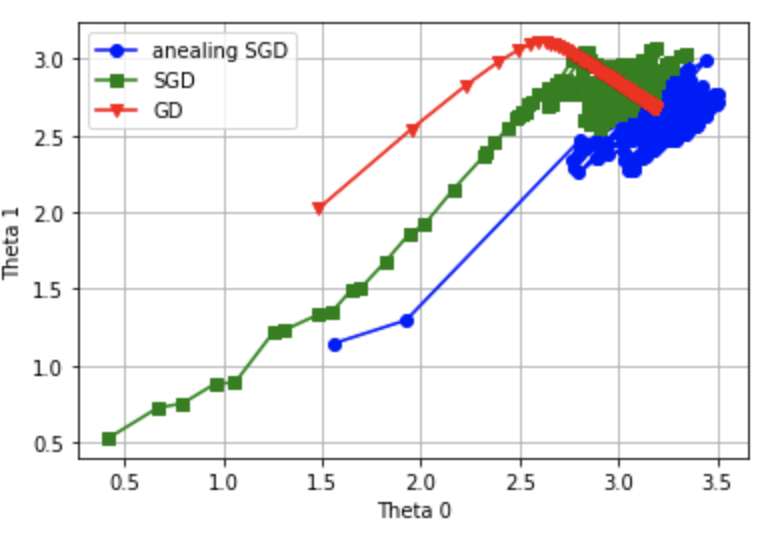
\includegraphics[scale=1.4]{sgd}}
            \caption{Visualzation of \emph{GD}, \emph{SGD}, and \emph{Simulated Anealing} characteristics}
            \label{fig_sgd}
        \end{figure}

        \hyperref[fig_sgd]{Figure \ref*{fig_sgd}} depicts the regression procedure of the three learning methods tested on a model with one attributes \footnote{As it has been discussed, $\theta_0$ is the bias.}. It can be seen that the basic \emph{GD} method becomes unefficient when it reaches near the minimum \footnote{The speed becomes much slower that before after the direction of $\theta_1$ changed at about 3.2.}. The \emph{SGD} has an undeterministic speed and it oscillates near the minimum. The \emph{Simulated Anealing} has a large speed at the beginning, and the speed is decayed as the iteration grows.

        \subsubsection{Polynomial linear regression model}
        When the linear regression can not have better fitness with the power of 1 for the attributes, the polynomial linear regression is introduced, with can extend the power of each feature to n.

        For example, for a vector $x = [a, b, c]$, if it is extended to degree $d = 2$, $x = [a, a^2, b, b^2, c, c^2, ab, ac, bc]$. The number of the attributes (n) will be extended to:
        \begin{equation}
            n_{poly}=\frac{(d+n)!}{d!\;n!}
        \end{equation}

        When the degree of the polynomial linear regression is increased, the cost function is becoming smaller, as the new degree applys more limitation on the model to well fit in the training set.

        There is also a trade-off between the degree and generalization of the model. As high degrees are easy to introduce overfitting, but that does not mean low degree is good. When the cost function can not decrease to an acceptable range no matter how much data has been fed, it is time to increase the degree. Low degree always introduces underfitting or high cost function.

        \subsection{Binomial regression}
        
        \section{Simulation frameworks}
        Two kinds of simulation frameworks have been considered in this project: \emph{event-driven simulation} and \emph{analytic simulation}.
        Both of them are introduced in this section.

        \subsection{\emph{Event-driven simulation}}
        This simulation framework is mostly used in circuit simulation software design. The basic idea is that the actions will trigger further events happen at a later time. Such events then also act as one action which can cause new events happen at a later time.
        This is a recursive procedure, which starts from an action and ends with all actions processed.

        To elaborate, think of an example from Harold \cite{book:sicp}. 

        \begin{figure}[ht]
            \centerline{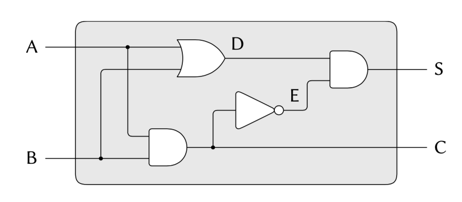
\includegraphics[scale=2.2]{halfadder}}
            \caption{An implementation of Half-adder}
            \label{figure_half_adder}
        \end{figure}

        \hyperref[figure_half_adder]{Figure \ref*{figure_half_adder}} shows a circuit of half adder linked using logical gates. Ports $A$ and $B$ are inputs representing two logical number to be added, $S$ is the sum, and $C$ is the carry. Its bool expression can be written as $S = (A|B)\&\overline{(A\&B)}, C = A\&B$. From both the expression, either a change of $A$ or $B$ will result in the changes on $S$ and $C$.
        Assume $A = 0$ and $B=0$, causing $S = 0$ and $C = 0$. At time $t=0$, $A$ is changed from $0$ to $1$. As $A$ is linked to \emph{OR-gate} D and \emph{AND-gate} F, this will drive the output of D to $1$ at a later time (an interval of \emph{OR-gate delay}). After the delay, the output of D changes to 1, this change becomes an action to the \emph{AND-gate} of $S$ and triggers a change after a \emph{AND-gate delay}.
        The wire $S$ has a new value after the delay, and the simulation system stops as there is no new action triggered by $S$.

        The key to this simulation scheme is a structure called \emph{Schema} \footnote{One implementation is a record of an integer value which represents the current time and a table of which the tuple is a record of an integer value which represents the specified time and a list of actions which are procedures on the wires. The wire can also be a record of a value and a list. The value is its current state: $0$ or $1$. The list is the actions added by each logical gates. So that when the value is changed by a start action or other trigerred events, the actions are performed to propagate the effects and trigger further events to the gates `after it'.}, which stores the information of the current time, and the \emph{agenda} which stores the actions that should be processed at a specified time. The simulation processing logic is to compare the current time and the specified time of the first \emph{agenda item} in the \emph{Schema}. If the two values are equal, process the actions in that \emph{agenda item}. If they are not equal, update the current time by an increase. After processing the the actions in one \emph{agenda item}, new actions may be added to be processed at a later time, and the current \emph{agenda item} is deleted. After the deletion, the originally second \emph{agenda item} becomes the first the \emph{agenda item} and the procedure calls itself at the end to perform a tail iteration. The procedure then run to the next \emph{agenda item} with the same logic till there are no \emph{agenda items} in the \emph{agenda table} which denotes the end of the simulation.

        Apart from the trigger propagation strategy, a log system is a necessary part of simulation framework, as it is the interface to the users to check simulation details and results. There are two available strategies: time-based log and event-based log. The differences can be understood from literal meaning that the time-based log records the state of each component on every time slot \footnote{Every time the current time in the \emph{Schema} is updated, the logger will record the states of all components. Thus, the time-based logger structure is a timetable.} and the event-based log records the information of a state change of one component \footnote{It can be embedded with the \emph{Event-driven} strategy as an action of the wire as a possible implementation. The structure is thus a diary.}. Generally, it is reluctantly to tell which is better, as the log can be converted or interpreted to the opposite form. It is the complexity of adding it to the specific simulation framework that causes the priority. For example, the lionized idea of the discussed digital circuit simulation system is based on \emph{Event-driven} strategy. A event-based logger system can be implemented by adding a new action called \emph{probe} which writes information of a state change to a log file whenever it is called. This new action is added to any wire to be logged and the details of log item can be changed by merely editing this action. However, if using the time-based log, the logger cannot be implemented as an action as the action is only called when it is triggered. It should be new structure which records each wire in the circuit. When the current time is updated in the \emph{Schema}, the logger procedure is launched to read this structure and record the state of each wire. Obviously, there are cumbersome codes to write for this logger.

        \begin{figure}[ht]
            \centering
            \begin{tikzpicture}[
                roundnode/.style={circle, draw=gray!80, fill=gray!15, very thick, minimum size=7mm},
                rectanglenode/.style={rectangle, rounded corners, draw=black, fill=gray!20, very thin, minimum size=5mm},
                rectanglenode2/.style={rectangle, rounded corners, draw=black, fill=white, very thin, minimum size=5mm},
                arrow/.style={thick,->,>=stealth}
                ]
                \node[rectanglenode, text width = 2.8cm] (firstnode) {\emph{main simulation process logic}};
                \node[rectanglenode] (secondnode) [below=0.6cm of firstnode.south] {Model components};
                \node[rectanglenode, inner xsep = 2.5cm, inner ysep = 0.7cm] (schema) [right=1cm of firstnode.east] {};
                \node at (schema.center) [above] {\emph{Schema}};
                \node[rectanglenode2] (currentTime)at (schema.base) [below left] {Current time};
                \node[rectanglenode2] (agenda) at (currentTime.east) [right=0.47cm] {\emph{agenda}};
                \node[rectanglenode, inner xsep = 2cm] (logger) [below=0.4cm of schema.south] {logger};
                \draw[arrow] (firstnode) -- (secondnode);
                \draw[arrow] (firstnode) -- (schema);
                \draw[arrow] (logger) -- (secondnode);
                \draw[arrow] (secondnode) -- (schema);
            \end{tikzpicture}
            \caption{Structure of \emph{Event-driven} simulation framework}
            \label{fig_structure_of_event_driven}
        \end{figure}

        \hyperref[fig_structure_of_event_driven]{Figure \ref*{fig_structure_of_event_driven}} shows the basic structure of a \emph{Event-driven} simulation system. Fow a power grid simulation system, the model components could be wind power generator, grid, EV, house, appliance. The state should be the time, because the consumption is assumed to be a function of time, for example, the household demand profile in \cite{report:household} is a function of time of the day, the season, the house type and house owner.

        \subsection{\emph{Analytic simulation}}
        Unlike the former strategy, this strategy is more generally applied, as its idea is easy to understand: analyze the model based on a some variables \footnote{Usually take the time as the variable, as most real-world model are based on time, or should be simulated by time.} for a specified amount of cycles. The core of this framework is the \emph{scheduler}, which intialize the model, run analytic functions for instructed number of cycles and terminate the model. It is like the \emph{Schema} in previous framework, but all of the actions have been determined before the simulation begin, and no new actions will be added during simulation. The action in the \emph{Analytic simulation} is called the \emph{Scheduled job} which is provided by the model.
        Take the power grid as an example. Models of grid, wind generation, house, EV and other objects in one grid should be implemented first, so that they can be added to the scheduler to be initialized. These models should contain an analytic function to be called on each simulation cycle by the scheduler, a termination function to be called at the end of the simulation, to summarize the results, such as the average value, the socre of special metrics.

        In this project, a simulation environment based on \emph{Analytic Simulation} called \emph{trick} \cite{website:trick} is used for simplicity. The reason is that it provides the interface of implementing model in \emph{C/C++}. Then the jobs can be scheduled using a script which includes the model and functions exposed to be called for intialization, analysis, and termination. Additionally, a versatile logger is provided. 

    \chapter{Work}
        \section{Establish a dataset from available source}
        A dataset is constructed to acquire understanding of power generation and demand in Orkney. The data set began to scrape data from 19th October. 
        This section describes the available data source used in this constructing the dataset and the details on implementation.

        \subsection{Data sources}
        The dataset contains data of three parts: generation and demand in Orkney, curtailment status in Orkney and the weather in Orkney.

            \subsubsection{Generation and demand data source}
            \label{text_generation_and_demand_data_source}
                The ANM website \cite{website:ANM} cosntains a bar chart to indicate the current power generation and demand of the whole
                island. Figure \ref{fig_anm_barchart} shows this chart. There are 5 records: Live Demand, Winter Peak Demand, Orkney ANM, Non-ANM Renewable Generarion, Total renewable capacity.
                Some explanations of them can be found in the left of the web page.
                However, the website itself dose not expose APIs to get these data, thus it is necessary to analyze its http request and response and use a 
                server to scrape the data periodically.

                \begin{figure}[ht]
                    \centerline{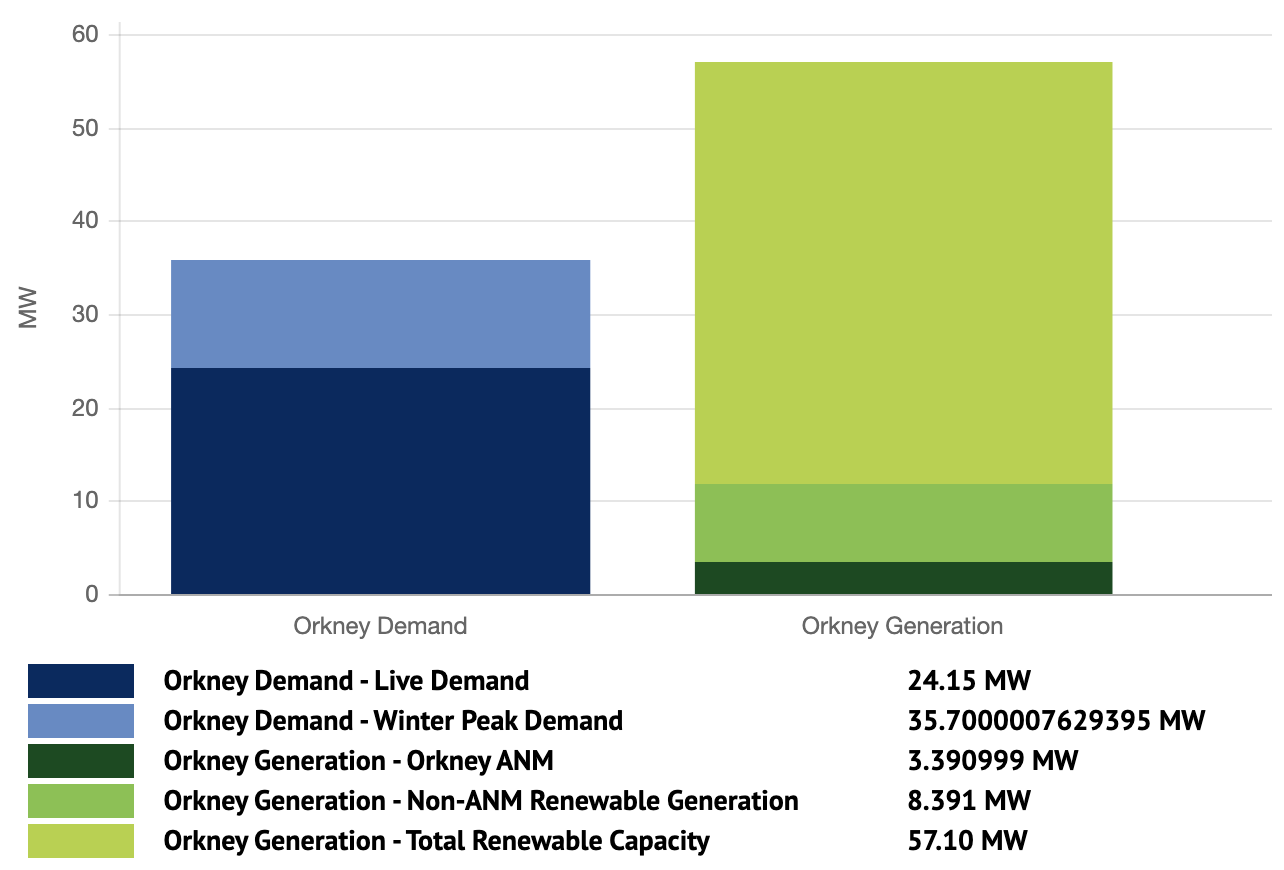
\includegraphics[scale=1]{anm_barchart}}
                    \caption{The Orkney Live bar chart to represent the energy generation and demand of the island}
                    \label{fig_anm_barchart}
                \end{figure}
            
            \subsubsection{Curtailment data source}
                On the ANM status website \cite{website:ANMstatus}, the island is divided into 9 zones as it is indicated in Figure \ref{fig_map}. Then there is a 
                table contains the current status of each zone. Unfortunately, there are neither public APIs to extract these data. The same method should
                be applied to scrape the data from this website.

                \begin{figure}[ht]
                    \centerline{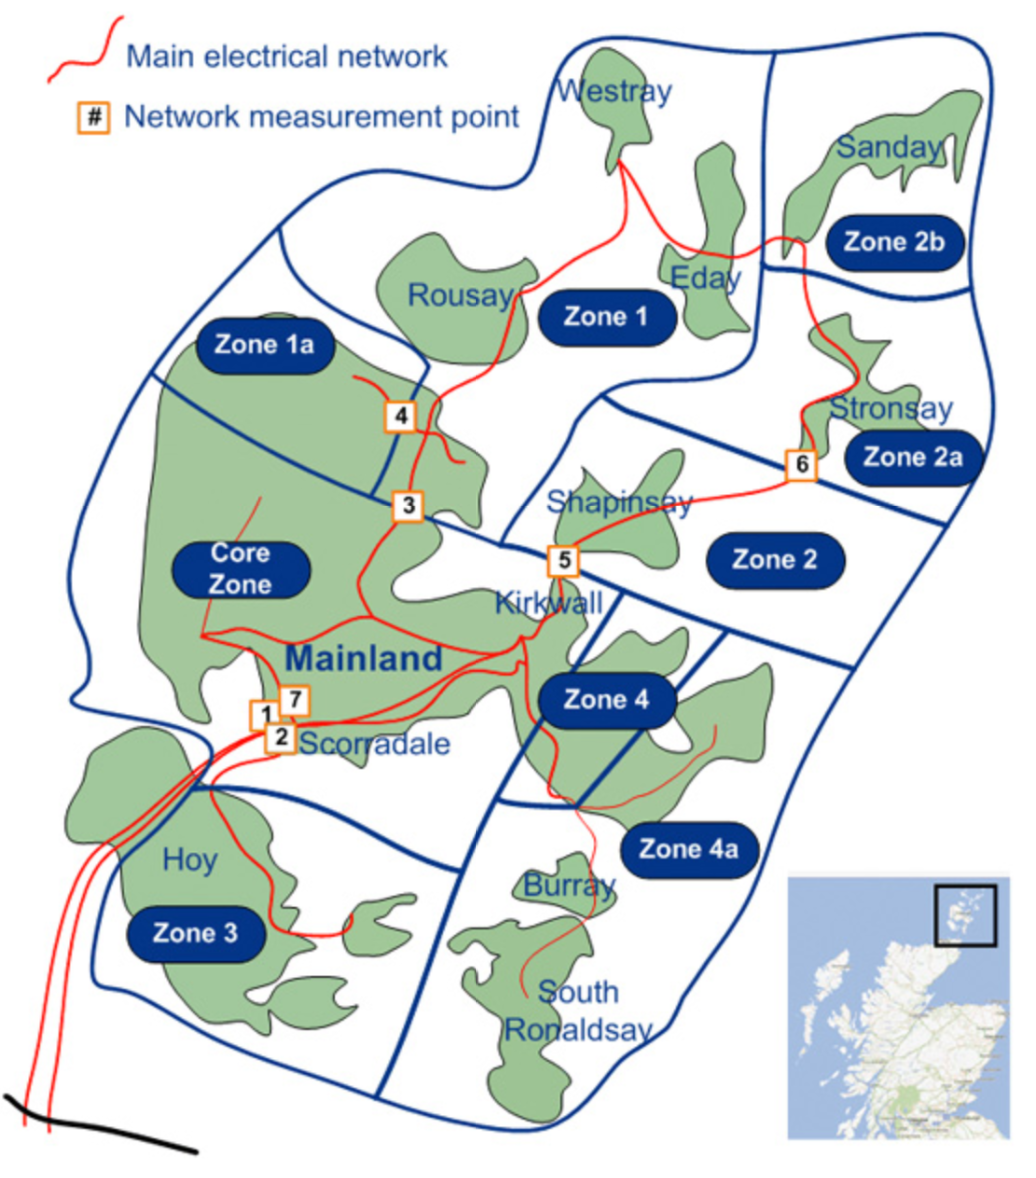
\includegraphics[scale=1]{map}}
                    \caption{ANM zones}
                    \label{fig_map}
                \end{figure}
            
            \subsubsection{Weather data source}
            \label{text_weather_data_source}
                The Open Weather Map website \cite{website:OpenWeatherMap} provides public APIs to clients to get weather information of all over the world.
                Depending on the functions, some APIs which can request for historical data are paid services and the free ones can only acquire data at current time point.
                As the former two sources are both extracted from real time, it is not necessary to get historical data. The free APIs are used to get the weather
                information in Orkney. Various kinds of weather information are available from this API, such as temperature, visibility, wind speed and degree, and clouds.
                As only the wind speed is directly related to wind power generation \cite{paper:Shao2010}, it is selected along with the temperature and humidity to be recorded in the dataset.
            
        \subsection{Tools and implementations}
        The dataset is established on a cloud server with Cent OS 7 installed. As the data needs to be requested periodically all the time, a cloud server is the most
        effiecient method. The scripts used in scrape the data are writen in python 3 \cite{website:python3} and bash \cite{website:bash}. Libaries and tools based in these two languages are mentioned below.

                \subsubsection{Fetching Generation and demand data}
                By tracing the http response and request, the from of the generation and demand data are transformed in a JSON format file. Then, it is possible to 
                use the Request python library \cite{website:requestpython} to immitate this http request and receive this file. After parsing the content, current power generation and demand data can
                be extracted and stored in the database built on the server. The store and program launch actions are controlled by crontab \cite{website:crontab} to execute in a 10-minute period.

                \subsubsection{Fetching curtailment data}
                \label{text_fetching_curtailment_data}
                The form of curtailment data is not JSON as it is embedded in the html file fetched from the request. The web page constains some javascript programs which demonstrate information
                on the table. Because this file is a mixture of programming logics and data, it cannot be analyzed using a JSON parser as the generation and demand data did. The method is that, first
                save this html file as a text file to the disk, then use grep \cite{website:grep} to find the clouses which contain the status data. The status data is again saved as a file. Relaunch
                a python script to parse this simplified file and store the data of the table to the local database. The Status of the zone is represented using 1s and 0s, as it is assumed that the state
                of each zone can only be off and on. Actually, there is one more state called partly off which was not noticed when writing the script file, thus only two states are recorded.

                \subsubsection{Fetching weather data}
                As the APIs are provided, the implementation is that to write a python script using a library which wrap the API functions of Open Weather Map in python \cite{website:pyowm}.
                Use the verification code provided after registering a client of the website and find the region code of Orkney, then the weather condition can be fetched in JSON format. Apply
                the same procedure are the power generation and demand data to store the weather data in the database.

                \subsubsection{Synchronizing database to local} 
                The database in the cloud server needs to be synchronized periodically to avoid possible loss due to abrupt. The method is to use github \cite{website:github}. Create a git reporsitory \cite{website:git}
                and add the database file into it. Then, use crontab to execute a push command of git to synchronize the repository on the remote server of github. To access the repository on remote server, it is mandatory
                to enter login id and password of a github user. As it is using crontab to synchronize, the interaction of git push will cause problems. The solution is to use the pexpect library \cite{website:pexpect}, which
                create a shell for each command needs interaction and interact with that command as the user defined. After solving this problem, the database can be updated without manualy controling extral steps. When it is
                needed for the user to get or update the dataset, directly pull the repository from github, as it is always synchronized to the clound server. The frequency of synchronization is set at 12:30 every day.

                \subsubsection{Data analyzing and visualizing}
                Various libraries are used. The Numpy and Scipy libraries \cite{website:numpy} \cite{website:scipy} are used to process statistical and vector-based computing. The Pandas library \cite{website:pandas} is used
                to loading dataset into memory and applying complex dataset enquiries. The Scikit-Learn library \cite{website:scikit} provides machine learning models and data preprocessing methods. The matplotlib library
                \cite{website:matplotlib} provides plotting and rendering tools to produce plot. These libraries all provide APIs in python. Thus, python programming language \cite{website:python3} is used. Another reason is that
                the task of data analyzing is generally classified to fast development, as the cycle of editing code and fatching the results must be short. The programming lauguage python \cite{website:python3}, which is a
                dynamically typed and script-based language, is satisfying all demands. Further more, the brower based programmable Jupyter notebook under Jupyter Project \cite{website:jupyter} provides a flexible and user-friendly
                UI for programming using python. This makes visualizing data like plots and tables in an easier and more efficient way.
                
        \subsection{Data bias and loss}
        It is definite that the data accuracy is limited under various reasons. No data sources listed above has the guarantees or warranties that the data is accurate, complete and up-to-date. 
        Since they are the only sources for Orkney, there are not other choices.

                \subsubsection{Sample loss}
                As it has been mentioned above, the sample rate is 10 minute. That is to say information between two neighboring sampling slots is out of observation.
                If some fierce disturbances happen at that interval, this information is lost because of low sampling rate. However, the ANM website does not provide
                the definition of the real-time data, nor data of each zones. Additionally, the data of the over-all island has been in aggragation pattern that cannot
                indicate spikes caused by individual household load or power generation. It is assumed that the information in each 10-minute interval is recoverable be
                observing its two neighboring samples.

                \subsubsection{Source stability}
                \label{text_source_stability}
                Under the assumed sample rate, there should be $6*24=144$ samples of each attribute each day. However, there are not always 144 samples in a one-day period.
                For example, the number of samples of the whole November should be $24*6*30=4320$, but the dataset only contains $4252$ samples. There are $68$ 10-minute samples
                lost. Additionally, from iterating these samples day by day, there are only two days satisfying the assumption of $144$ samples a day. Most of the days contain
                $141$ or $142$ samples. The reason is that the ANM website always runs into corruption: the website cannot response to the requests and accessing through browser results
                in another page of maintenance. It seems that it will become unresponding for a very short period each day from the samples. However, it is recorded that the website
                went to a longer corruption from 13th December to 19th December and 25th January to 29th January.

                The methods of analyzing data of time series in this project are all designed under the presumption that there are no samples lost. The days with not enough samples cannot be
                used sequenctially. However, if only several days with enough samples are used, there will be only two days in November. The defact of most of the days is just the missing on
                one or two samples. Thus, it is possible to recover these lost samples from linear prediction of samples before and after the point. A method of fix these loss points is discussed
                in Data cleaning section. Under the condition that the sample of half or the whole day is lost, there is not possible ways to recover, thus, these days are excluded from
                analysis.
            
                
        \section{Orkney over-all demand analysis}
        Based on the data of over-all Orkney demand, a demand profile can be analyzed using techniques on aggragation and smoothing. This profile provides a bird view of daily demand pattern in Orkney.
        In this section, the details of analysis of demand data in Orkney is discussed.

                \subsection{The attributes of demand}
                \label{text_attributs_of_demand}
                As it has been recorded in section \ref{text_generation_and_demand_data_source}, there are two demand attricutes in the dataset: Live demand, Winter peak demand. From literal sense, the 
                Live demand could be the demand of current time and the Winter peak demand could be an estimation of current maximum demand based on historical data or learning models. There is no explanation
                on thw website of them.
                
                Actually, the two attributes can be added to one constant, which is demonstrated in Table \ref{table_demands_properties}, where the mean, standard deviation, and various percentiles have been calculated.
                The sum attribute is calculated by adding the two demand attributes and it becomes a constant over all time.

                
                \begin{table}[ht]
                    \centering
                    \begin{tabulary}{\linewidth}{c c c c}
                        \hline
                         & Live Demand & Winter Peak Demand & Sum \\ \hline
                        \hline
                        mean & 19.04 & 16.66 & 35.7 \\ \hline
                        std & 2.92 & 2.92 & 0 \\ \hline
                        min & 10.57 & 8.05 & 35.7 \\ \hline
                        25\% & 16.91 & 14.52 & 35.7 \\ \hline
                        50\% & 18.9 & 16.8 & 35.7 \\ \hline
                        75\% & 21.18 & 18.79 & 35.7 \\ \hline
                        max & 27.65 & 25.13 & 35.7 \\
                        \hline
                    \end{tabulary}
                    \caption{Statistical properties of two demand attributes and their sum}
                    \label{table_demands_properties}
                \end{table}

                The Winter peak demand attribute is taken out of consideration. One reason is that it can be calculated from the sum $35.7$. The other reason is that
                the peak value is even lower than the Live demand. Curiously, the implication of why ANM chooses to use this attribute is impossible to understand; on the one hand,
                the live demand has been enough to represent the load of the grid on the island, on the other hand, the peak demand is not the peak demand in strict sense.
                The analysis on demand will thus only focus on the Live Demand.

                \subsection{Weekday profile}
                The first step of analyzing demand is to classify them into weekdays. The reason is that, intuitively, the demand is determined by individuals' behaviors, their behavors
                have disciplines under the routine plans. For example, a white collar gets up at 7:00 in the morning, he opens the oven to cook food, then this will result in a consumption
                increase in the morning, he goes to company, turns on his computer and prepares coffee, this forms a consumption by computer and pot. At night, he watches TV, then takes a shower, this
                results in audiovisual and heating consumption. This description implies that specific vocation has generate demand under defined pattern. Generally, most of people work in the day and 
                stay at home at night. They take meals and go to sleep at the same intervals so that these consumptions appear significantly in the over-all demand. The possible differences should be
                that the behaviors are different on various weekdays.

                Take the demand of all mondays from the end of October and the whole November as the first group to be analyzed. If all these mondays are workdays or citizens' behaviors are
                enough disciplinary, large degree of correlation should be able to be acquied and the standard cross-correlation should tend to 1 to demonstrate large relation. That is to say, 
                the demands of these days increase and decrease at the same time which appear to be similar patterns. If this is true,
                the assumption to build weekday profile is reasonable, and the aggregated demand trace can be calculated using the average value of these days. Then, profiles of other weekdays can be analyzed using the same method.

                The extracted mondays are 10-22, 10-29, 11-05, 11-12, 11-19, 11-26. Using these six days, first calculate the their correlation matrix \footnote{A correlation matrix is a table showing correlation coefficients between variables. Each cell in the table shows the correlation between two variables.}.
                Table \ref{table_correlation_matrix_monday_demand} records correlation matrix of the six days calculated using `\emph{corrcoef}' method of Numpy. From this matrix, two days are to be specially paid attention to: 10-22, 11-19. The 10-22 demand appears to be negatively correlated to other days expcept 11-19, and the 11-19 data is positively correlated with all other days under low degrees \footnote{From experience, the standard correlation value larger than 0.7 can be detected with large similarity}. While other days can be characterized as largely similar from their high correlation values.

                \begin{table}[ht]
                    \label{table_correlation_matrix_monday_demand}
                    \centering
                    \begin{tabulary}{\linewidth}{c | c c c c c c}
                        \hline
                         & 10-22& 10-29& 11-05& 11-12& 11-19& 11-26 \\ 
                        \hline
                        10-22 & 1 & -0.48 & -0.59 & -0.49 & -0.35 & -0.34 \\
                        10-29 & -0.48 & 1 & 0.77 & 0.88 & 0.30 & 0.63 \\
                        11-05 & -0.59 & 0.77 & 1 & 0.83 & 0.34 & 0.76 \\
                        11-12 & -0.49 & 0.88 & 0.83 & 1 & 0.22 & 0.61 \\
                        11-19 & -0.35 & 0.30 & 0.34 & 0.22 & 1 & 0.61 \\
                        11-26 & -0.34 & 0.63 & 0.76 & 0.61 & 0.61 & 1 \\
                        \hline
                    \end{tabulary}
                    \caption{The correlation matrix of Monday demand data}
                \end{table}

                The problem should be more obvious if the six days are plotted in one graph in one-day interval. Figure \ref{plot_monday_demand} depicts the data of these six days and also the average of thier sum as the aggregated data. The four days characterized as largely similar above have most of the time point coinciding, and the two days defined as outliers have significant differences with the common pattern and are emphasized using red colored rectangle. The 10-22 data has a very low level in the afternoon, and inversely, the 11-19 data has a much higher consumption in the morning. Those are what effect the correlation scores. Though, these two days have shown different patterns of mondays, the aggregated sum is not largely influenced, as it is coinciding with other four days in the graph. Therefore, if most of the days of Monday adhere to the main pattern, then the outliers cannot interfere the aggregation.

                \begin{figure}[ht]
                    \label{plot_monday_demand}
                    \centerline{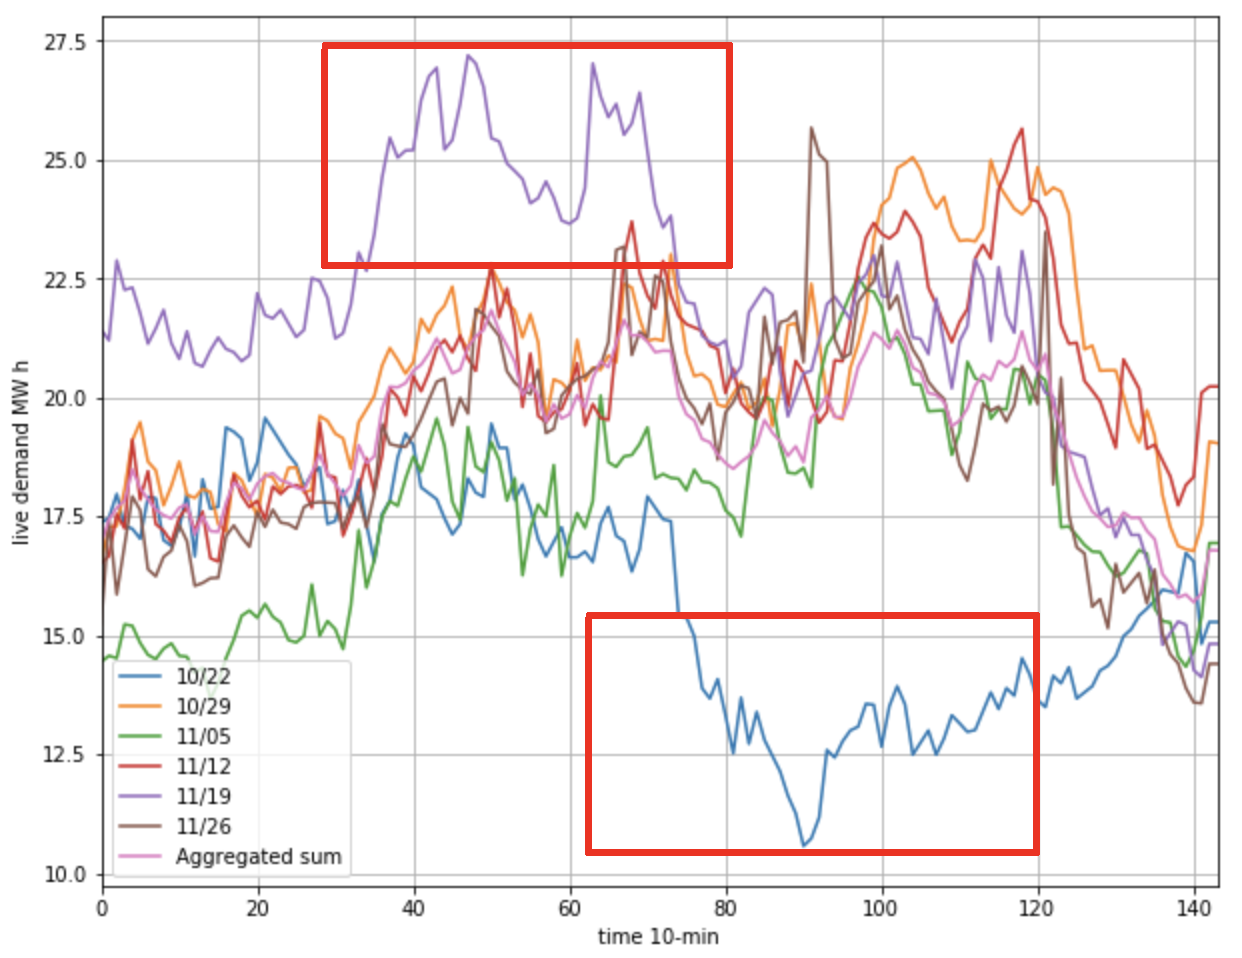
\includegraphics[scale=0.27]{monday_demand}}
                    \caption{The demand of mondays and their aggregated sum in one-day period, the differences of two outliers are specially selected}
                \end{figure}

                There should be reasons to explain the abnormal pattern on 10-22 and 11-19, however, no valid news or information can be found through web on these two days in Orkney. There must be something happen, for example, a maintenance which results in a lot of households turning off the appliances or a festival which increase the demand. Because 10-22 has lower average demand and 11-19 has larger average demand, and both of the days have larger standard deviations. The details of means and standard deviations are shown in Table \ref{table_mean_std_monday}.It should be viable to infer the two special conditions.

                \begin{table}[ht]
                    \label{table_mean_std_monday}
                    \centering
                    \begin{tabulary}{\linewidth}{c |c c c c c c c}
                        \hline
                         & 10-22 & 10-29 & 11-05 & 11-12 & 11-19 & 11-26 & Aggregation\\ \hline
                        % \hline
                        Mean & 15.82 & 20.68 & 17.67 & 20.31 & 21.83 & 19.05 & 19.23\\
                        Standard deviation & 2.31 & 2.18 & 2.18 & 2.09 &2.86 & 2.43 & 1.5\\
                        \hline
                    \end{tabulary}
                    \caption{Mean and standard deviation of six Mondays}
                \end{table}

                From Table \ref{table_demands_properties}, the average demand and the standard deviation in a global scope are 19.04 MW h and 2.92, and the four normal days have their means near to the global value, while the two outliers have larger differences. The aggregation data also has a closer average, the deviation is lower adhere to \emph{Variance} \footnote{For the sample average of i.i.d.:  $S_n = (X_1 + \dots + X_n)/n$, the deviation \\$\sigma_n^2 = \sigma^2/n$}.
                A more clean plot can be viewed in Figure \ref{plot_monday_agg}, where only the aggregated data and the mean is plotted. From the plot, it can be identified that there are four peak demand periods at almost the same level on the Monday, and they demonstrate the people's behaviors in the morning, noon, afternoon and evening.
                If 7:00 am - 8:00 pm (42 - 120 10-minute) is defined as the diurnal interval, most of consumption in this period will be over the mean consumption. Then the compliment of this period, the nocturnal period, has energy consumption lower than the average in most of the time.
                \begin{figure}[ht]
                    \centerline{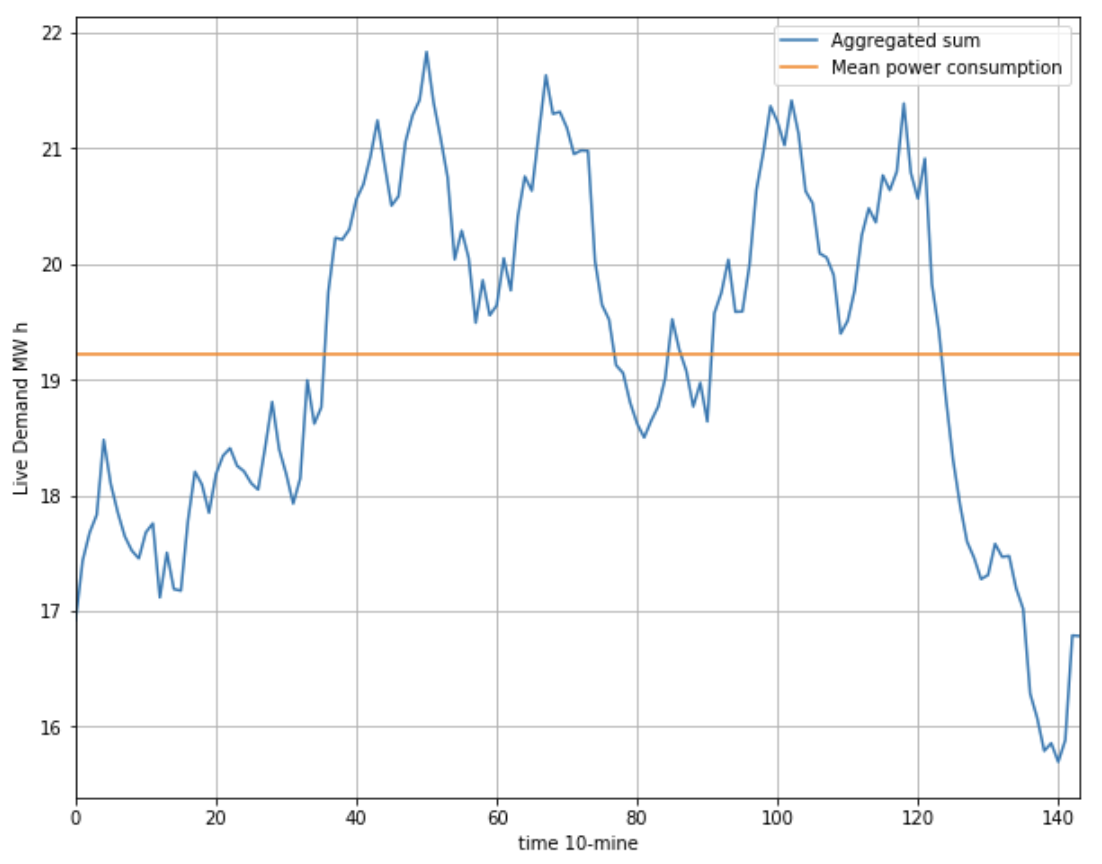
\includegraphics[scale=1.2]{monday_agg}}
                    \caption{The plot of Aggregation sum and its mean of Monday}
                    \label{plot_monday_agg}
                \end{figure}

                The next step is to apply this analysis method to each weekday. From the assumption and the experience of the Monday case, there will be some outliers in each weekday though, most weekdays appear a similar pattern and they are indicating the main tendency of demand. The date range is selected to be the whole November, as the dataset was established at 19th October, and there are long term data loss in December and January \ref{text_source_stability}. The data is first classified by seven weekdays, then apply aggregation to each weekday group. Finally, the seven aggregation weekdays are plotted and analyzed to find their similar patterns.

                \begin{table}[ht]
                    \centering
                    \begin{tabulary}{\linewidth}{c |c c c c c c c}
                        \hline
                         & Sunday & Monday & Tuesday & Wednesday & Thursday & Friday & Saturday \\ \hline
                        % \hline
                        Sunday & 1 & 0.96 & 0.93 & 0.93 & 0.98 & 0.94 & 0.84 \\
                        Monday & 0.96 & 1 & 0.97 & 0.94 & 0.94 & 0.90 & 0.80 \\
                        Tuesday & 0.93 & 0.97 & 1 & 0.95 & 0.93 & 0.90 & 0.79 \\
                        Wednesday & 0.93 & 0.94 & 0.95 & 1 & 0.93 & 0.90 & 0.81 \\
                        Thursday & 0.98 & 0.94 & 0.93 & 0.93 & 1 & 0.92 & 0.81 \\
                        Friday & 0.94 & 0.90 & 0.90 & 0.90 & 0.92 & 1 & 0.95 \\
                        Saturday & 0.84 & 0.80 & 0.79 & 0.81 & 0.81 & 0.95 & 1 \\
                        \hline
                    \end{tabulary}
                    \caption{Correlation matrix of weekdays' aggregation on November Live demand}
                    \label{table_corr_weekday_demand}
                \end{table}

                Table \ref{table_corr_weekday_demand} shows the correlation matrix of the seven aggregations. As most of them are over 0.9, the profile of each weekday appears to be similar in large degree and it implies that they can be aggregated for the second time to form a new aggregation of the month. What can be verified is that the demand pattern of a day in Orkney is always following a similar pattern, the value may at a degree though, the peak value and the lowest value can always occur at the same time. This result should be implicitly true before the experiment, as this is the overall demand data, which records the total electricity demand of the island to represents the behavior of most people in common.
                
                \begin{figure}[ht]
                    \centerline{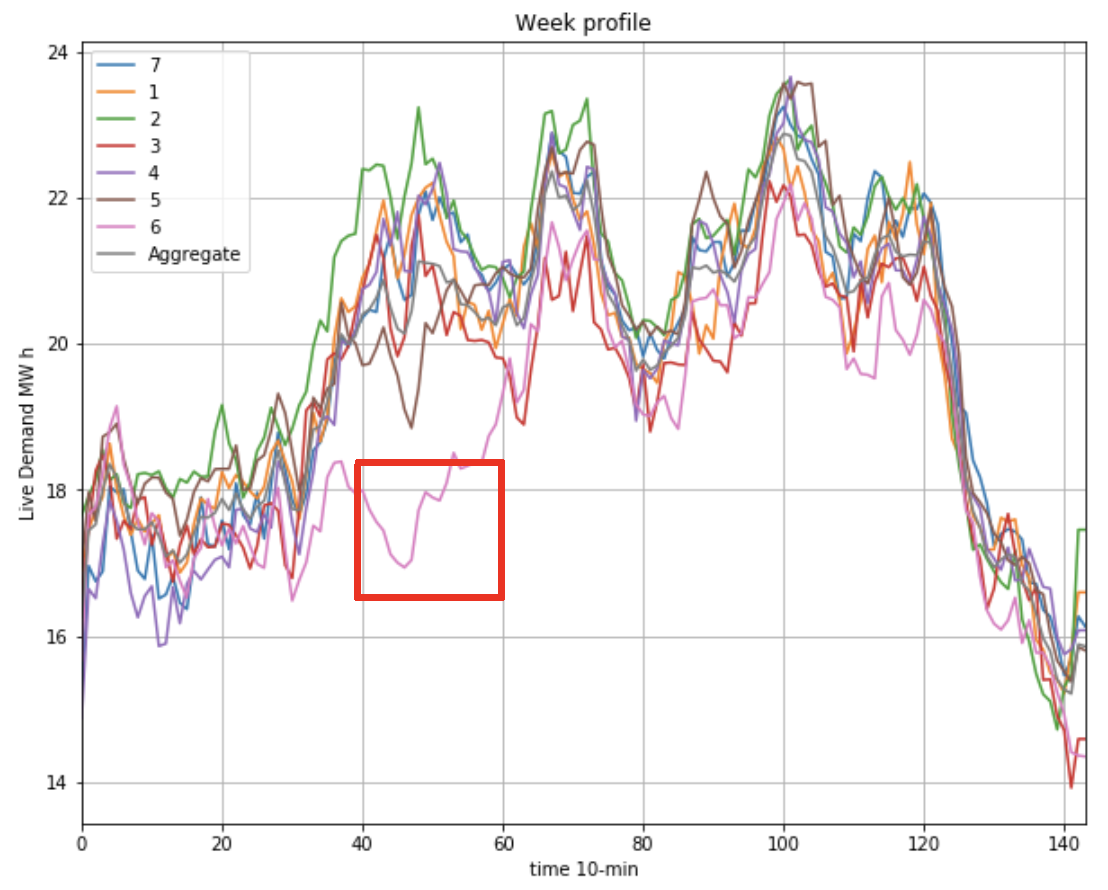
\includegraphics[scale=1.4]{weekday_profile}}
                    \caption{The aggregations of demand in 7 weekdays of November and the aggregation of the month}
                    \label{plot_week_profile}
                \end{figure}
                
                Figure \ref{plot_week_profile} shows a plot of the seven aggregation data to visualize their similarity. A discrepancy of them is at the red colored rectangle, where the demand of Saturday in the morning is lower. it can be verified from the correlation matrix that the scores for Saturday (at the bottom row) is lower about 0.1 than those of other weekdays on average. Except this disagreement, other aggregations appear to be largely similar and seem to follow the same path of growing and decaying during a day period. The aggregation of these seven weekday profiles is thus following the same pattern of the day.

                \subsection{Month profile}

                As it is mentioned in the last section, a profile of the month can be made using the aggregation of each weekday which is actually the aggregation of each day in the month. The reason is that the results of the aggregations of each weekday appear highly correlated, so that a new aggregation can be calculated based on this result. Apart from the behaviors in a day definition, the behaviors in a season definition can differ in various ways. The most general case is the heat is the heating consumption which is approximitely zero in the summer but has a large load profile in the winter. \hyperref[plot_heating_season_effect]{Figure \ref*{plot_heating_season_effect}} shows the seasonal effect on heating appliances which is collected from \cite{report:household}. The factor can reach about 3.0 in January and drop to 0 in summer monthes, thus causing big variances for month profiles in different seasons.

                \begin{figure}[ht]
                    \centerline{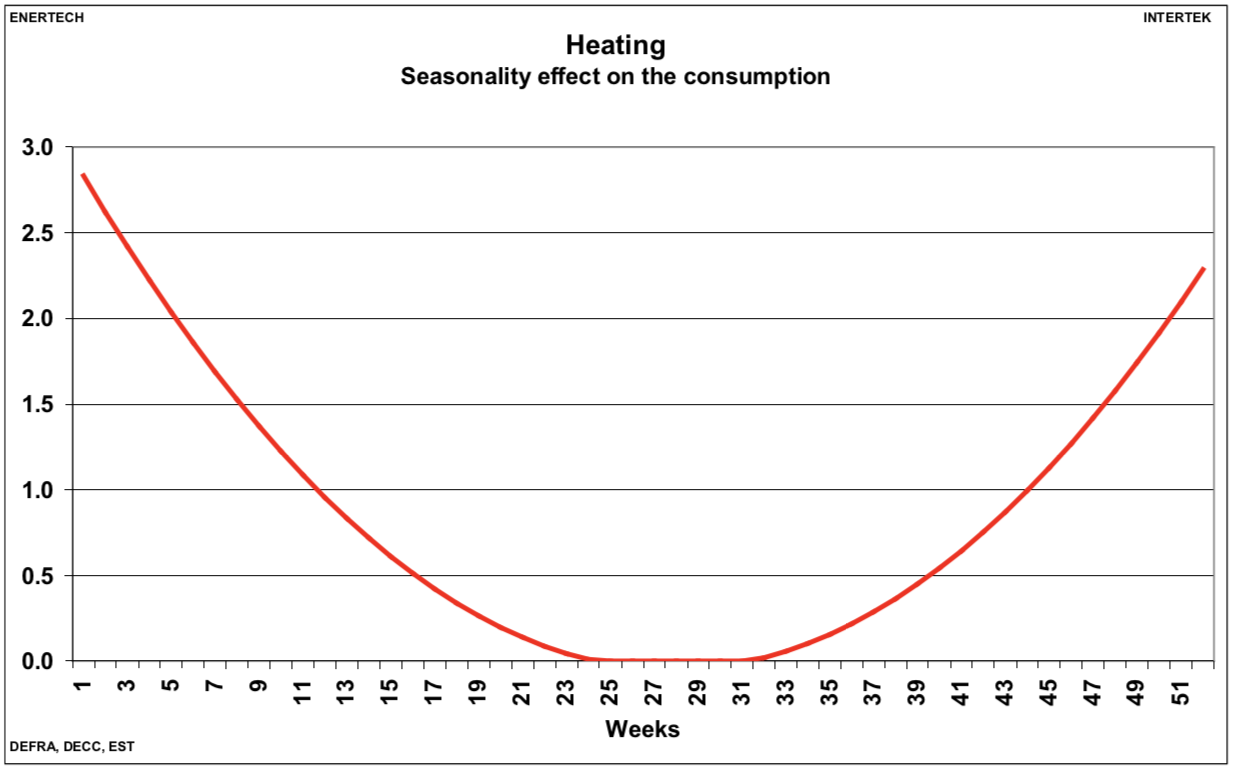
\includegraphics[scale=1]{heating_season_effect}}
                    \caption{Seasonal effect of heating}
                    \label{plot_heating_season_effect}
                \end{figure}

                \subsection{The month profile of November}
                    Limited by the coverage of dataset that it is collected in late October and huge corruptions happened in December and January (in \hyperref[text_source_stability]{Section \ref*{text_source_stability}}), the current available month profile analysis can only be applied to November. Additionally, the overview of this month has been enough for later analysis on the effects of EVs.
                    \hyperref[plot_november_demand_profile]{Figure \ref*{plot_november_demand_profile}} shows the final aggregation demand profile of November with three constant patterns: 21.9, 20.2, 17.7.

                    \begin{figure}[ht]
                        \centerline{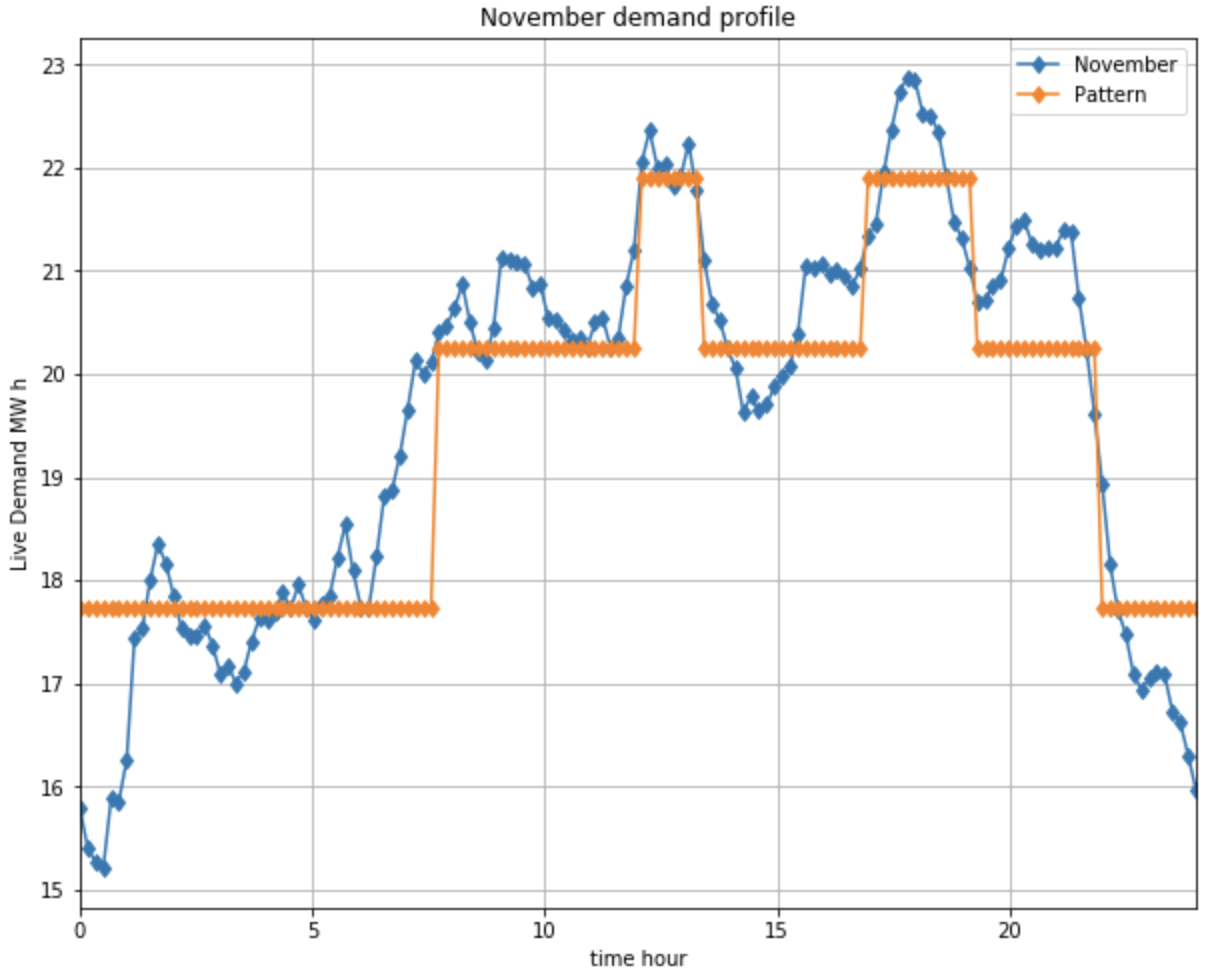
\includegraphics[scale=1]{november_demand_profile}}
                        \caption{The aggregated demand profile of November}
                        \label{plot_november_demand_profile}
                    \end{figure}
                
        \section{Orkney Wind generation analysis}
        The wind power generation analysis is fundamental to this project of building a generation-to-demand model. This analysis will provide statistical wind power characteristics and real-time cases for later simulation. In this section, the ANM record of wind power generation is first discussed, then a linear regression model will be created to link wind speed with wind power generation with curtailment introduced.

                \subsection{The power generation attributes}
                As it has been mentioned in \hyperref[text_generation_and_demand_data_source]{Section \ref*{text_generation_and_demand_data_source}}, there are three attributes relating to the power generation: Orkney ANM, Non-ANM Renewable Generarion, Total renewable capacity. The Orkney ANM is indicating the power generation from ANM system, and the Non-ANM Renewable Generation is the generation which is not controlled by ANM. As it is recorded in \cite{report:OrkneyAudit}, there are three kinds of \\connections of generation to grid. The Total renewable capacity should be the estimated full load generation at current time from its literal meaning. Adding the first two attributes as the Total generation to compare to the capacity by statistical characteristics. \hyperref[table_statistical_characteristics_generation]{Table \ref*{table_statistical_characteristics_generation}} shows their statistical characteristics, where Total \\Generation has the same standard deviation as Total Renewable Capacity, implying that they are vibrating at the same amplitude. This condition is similar to \hyperref[text_attributs_of_demand]{Section \ref*{text_attributs_of_demand}}, where the Peak Winter Demand and Live Demand can be added up to a constant at each point. Thus, the sum and subtraction of Total Generation and Total Renewable Capacity are performed as the Sum and Subtraction attributes in the table. As previously inferred, their sum appears to be a constant again. It is preposterous that the ANM choose to use these two attributes which can always be calculated from others, nor are their names misleading the readers.
                \begin{table}[ht]
                    \centering
                    % using @{\hspace{0.09\linewidth}} to change width of the column
                    % finally choose to use p attributes to coordinate mannually
                    \begin{tabulary}{\linewidth}{c p{1.7cm} p{2cm} p{2cm} p{2cm} p{1.1cm} L}
                        \hline
                         & Orkney ANM & Non-ANM Renewable Generation & Total Generation & Total Renewable Capacity & Sum & Sub \\ \hline
                        % \hline
                        mean & 10.09 & 12.43 & 22.52 & 34.58 & 12.07 & 57.1 \\
                        std & 6.92 & 6.99 & 13.54 & 13.54 & 27.08 & 0 \\
                        min & -2.09 & 0.26 & -1.53 & 15.08 & -26.95 & 57.1 \\
                        25\% & 2.89 & 5.40 & 8.32 & 22.25 & -12.61 & 57.1 \\
                        50\% & 11.23 & 14.73 & 27.25 & 29.85 & 2.61 & 57.1 \\
                        75\% & 16.54 & 18.47 & 34.85 & 48.78 & 40.46 & 57.1 \\
                        max & 21.26 & 25.96 & 42.02 & 58.63 & 60.17 & 57.1 \\
                        \hline
                    \end{tabulary}
                    \caption{Statistical characteristics of Generation attributes}
                    \label{table_statistical_characteristics_generation}
                \end{table}

                Originally, another explanation is assumed that the Total Renewable Capacity attribute is the estimation of the available capacity of storage to the grid. There are two reasons to refute this position. One is that the ANM network has been commissioning no battery storage since 2015 and the only available storage is the hydrogen fuel installed by \emph{Surf`n'Turf} \cite{report:OrkneyAudit}. The other reason is that the storage should be represented by energy not power and even if it is represented using power, the mean, which is 15.07 from \hyperref[table_statistical_characteristics_generation]{Table \ref*{table_statistical_characteristics_generation}}, is not reasonable. Because the wind is strong in Orkney and there is 61\% of the time the generation is higher than the demand. This implies that the battery should be at approximitely full storage for most of the time. Having proved that Total Renewable Capacity is of nonsense, the two renewable generation attributes are applied to an additive operation on element wise to form a Total Generation attribute, as they are both renewable generations installed by different sponsors.

                \subsection{The weather attributes}
                \label{text_wind_speed_analysis}
                As it is discussed in \hyperref[text_weather_data_source]{Section \ref*{text_weather_data_source}} that wind speed, temperature and humidity attributes are recorded in the dataset, a first attempt is on the wind speed for its strong relation to wind power generation.
                \hyperref[table_wind_speed_characteristics]{Table \ref*{table_wind_speed_characteristics}} shows the wind speed characteristics. Though the average speed is 6.01 m/s, the max value can reach 19.5 m/s,
                which must be identified as extreme weather. The 50 percentiles reach only 5.7 m/s, indicating that about half of the days have smaller wind speed than the average. However, the 75 percentiles construct
                a strong wind group with larger deviation than other intervals, implying the various conditions of wind, which result in challenges for the wind generation.

                \begin{table}[ht]
                    \centering
                    \begin{tabulary}{\linewidth}{C C C C C C C}
                        \hline
                        Mean & Std & Min & 25\% & 50\% & 75\% & Max \\ \hline
                        \hline
                        6.01 & 3.42 & 0.5 & 3.1 & 5.7 & 8.2 & 19.5 \\
                        \hline
                    \end{tabulary}
                    \caption{Wind speed statistical characteristics}
                    \label{table_wind_speed_characteristics}
                \end{table}

                Another special scenario of wind speed is its distribution. From the data of Orkney, the mean of is more near to the min than the max. If it is subtracted by two standard deviation, it will be a minus value and it is impossible. While the adding of two standard deviation is possible and it results in at least 75 percentiles, which is adhere to \emph{Chebyshev's Inequality} \footnote{In probability theory, Chebyshev's inequality (also called the Bienaymé–Chebyshev inequality) guarantees that, for a wide class of probability distributions, no more than a certain fraction of values can be more than a certain distance from the mean. \\ $\Pr(|X-\mu| \ge k \sigma) \le \frac{1}{k^2}$ \cite{website:chebyshev}} to be smaller than 0.25.
                The distribution is \emph{Weibull distribution} \cite{paper:windstructure}, which is a modified version of the general \emph{Rayleigh distribution}.

                \subsection{The curtailment attributes}
                The curtailment data is collected as binary type in \hyperref[text_fetching_curtailment_data]{Section \ref*{text_fetching_curtailment_data}}. There are three kinds of issues in a zone: ANM Operation, SHEPD Equipment, Generator Site Issue. For the sake of simplisity, the curtailment of one zone is the result of any issues in the zone.

                \subsection{Linking wind power genration to wind speed and curtailment}
                The difficulty of this problem is that the influence of the other attribute cannot be removed while analyzing one attribute. For example, the wind power increases along with the growth of wind speed, it then reaches a maximum limited by the largest rotation speed of the wind turbines. Thus, the model of generation should first increase linearly with wind speed, then appears horizontally at higher wind speed. With the addtion of curtailment, the model reaches the maximum level earlier and even the generation with lower wind speed is affected, as the curtailments happen whenever the generation exceeds the demand to some degree.
                It is thus possible to make a regression model which is allowed to under-estimate the generation.
                \label{text_wind_regression_model}
                    \subsubsection{The sample data}
                    It is deeply acknowledged that the data matters more than algorithms in machine learning, which is discussed in \cite{paper:datasize}. However, the data size of this model is just from one day which is specifically selected to demonstrate the main feature of wind speed to generation.
                    As it is depicted in \hyperref[plot_speed_vs_power_1202]{Figure \ref*{plot_speed_vs_power_1202}} that 12-02 is selected as the sample source. The reason is that an apparent linear relation of wind speed to generation and the upper limitation can be detected in the figure.
                    It can be found that the the generation grows linearly reciprocal to the wind speed before the wind speed reaches 8 m/s. Then it stops at about 38 WM h. The red line in the figure depicts the expected generation characteristics.

                    \begin{figure}[ht]
                        \centerline{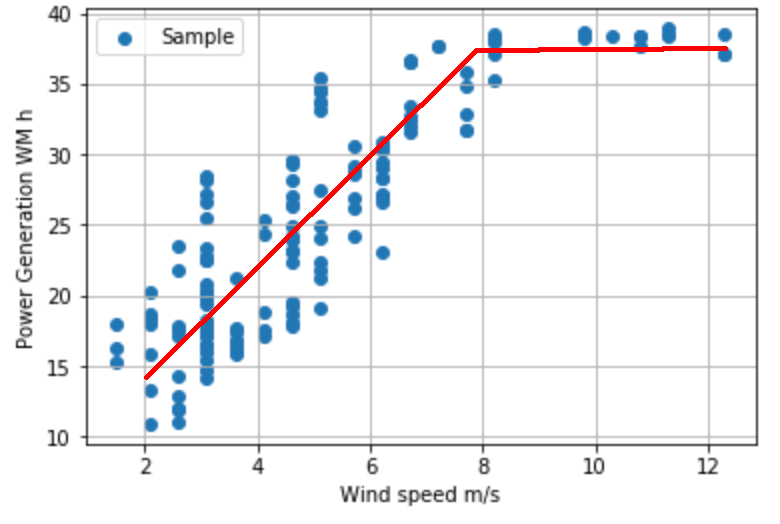
\includegraphics[scale=1.4]{powervsgenerationsample}}
                        \caption{The wind speed versus power generation on 12-02}
                        \label{plot_speed_vs_power_1202}
                    \end{figure}
                
                    If the whole dataset is selected, as \hyperref[plot_speed_vs_power_whole]{Figure \ref*{plot_speed_vs_power_whole}} indicated, various curtailment conditions will definitely affect the model. As the red colored rectangle emphasized, the value generation of 2.5 m/s to 7.5 m/s has approximitely the same range of value which cannot be appropriately understood by the algorithms.

                    \begin{figure}[ht]
                        \centerline{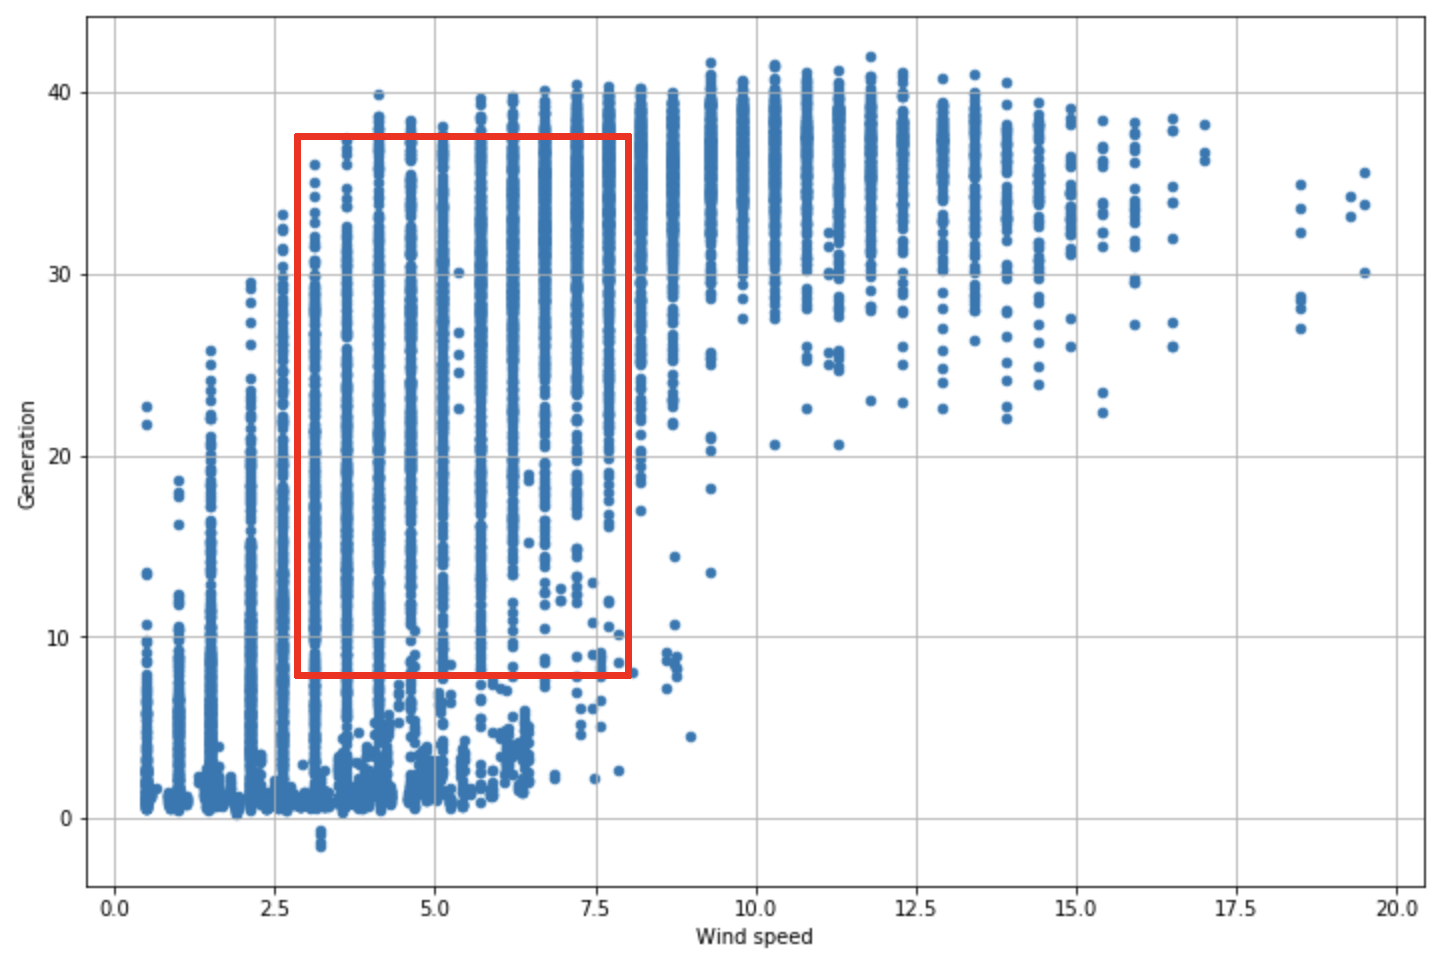
\includegraphics[scale=0.2]{generationvsspeedwholeset}}
                        \caption{The wind speed versus power generation on the whole dataset}
                        \label{plot_speed_vs_power_whole}
                    \end{figure}

            \section{Over-all EV effects}
                \subsection{Characterize EV charging events}
                \subsection{Analyze different penetration level}
            
            \section{Implementing the simulation model of the grid}
                \subsection{Simulating Household load}
                \subsection{Simulating EV charging load}
                \subsection{Simulating wind generation}
                \subsection{Simulating grid storage}
            \section{Determination of storage}

    \chapter{Conclusion}
    %The last chapter of your report must cover the conclusions. You discuss (briefly) the problems that arose which you had not anticipated, and how, as a result of this knowledge you would change the project. You discuss the projects limitations and discuss how these may be overcome. In short, you are clarifying the situation for the person who shall follow you and continue the project by pointing out where he needs to direct most of his efforts. As the project is only intended to create a prototype (except in certain special circumstances) there should be many useful modifications which you can suggest, and much from what you have experienced in your project work that you can impart to others. Consequently, of all the chapters in your report, the conclusions are probably the ones which best portrays your ability as an engineer.
    \chapter*{Appendices}
    \addcontentsline{toc}{chapter}{Appendices}
    \cleardoublepage  
    \phantomsection  
    \addcontentsline{toc}{chapter}{Bibliography}
    \bibliographystyle{IEEEtran}
    \bibliography{dissertation}
\end{document}